\documentclass{article}
\usepackage{amsmath, amssymb, amsthm, amsfonts, bm}
\theoremstyle{remark}
\newtheorem*{theorem}{Theorem}
\newtheorem*{remark}{Remark}
\newtheorem*{definition}{Definition}
\newtheorem*{hypothesis}{Hypothesis}
\newtheorem*{corollary}{Corollary}
\theoremstyle{remark}

\usepackage{physics}
\usepackage[a4paper, total={6in,10in}]{geometry}
\usepackage[dvipsnames]{xcolor}
\usepackage{hyperref}
    \hypersetup{colorlinks=true, linkcolor=ForestGreen}
\usepackage{graphicx}
    \graphicspath{{./img/}}
\usepackage{tikz}
\usepackage{ragged2e}
\usepackage{array}   % for \newcolumntype macro
\newcolumntype{L}{>{$}c<{$}} % math-mode version of "l" column type

\usepackage{soul}

\newcommand{\where}[1]{\begin{flushright}where #1.\end{flushright}}
\newcommand{\wher}[1]{\begin{flushright}#1.\end{flushright}}
\newcommand{\mylabel}[2]{\hyperref[#1]{#2}\label{back:#1}}
\newcommand{\myref}[1]{\hyperref[back:#1]{$\bigstar$}\label{#1}}
\newcommand{\e}{\hat{\vb{e}}}  % unit vector
\newcommand{\s}[1]{\textsubscript{#1}}
\everymath{\displaystyle}
\begin{document}

\begin{enumerate}
    \item $\vb{E}(\vb{r}) = \frac{1}{4\pi\epsilon_0}\frac{q}{r^2}\vb{\hat{r}} $
    \item $\curl\vb{E}(\vb{r}) = 0 $
    \item $\vb{E}(\vb{r}) = -\grad V(\vb{r}) = -\left(\vb{\hat r}\pdv{r}+\vb{\hat \theta}\frac{1}{r}\pdv{\theta}\right) $
    \item Electric dipole moment $\vb{p}\equiv q\vb{a} $
    \item $V(r,\theta) = \frac{1}{4\pi\epsilon_0}\frac{p\cos\theta}{r^2} = \frac{1}{4\pi\epsilon_0}\frac{\vb{p}\cdot\vb{\hat r}}{r^2} $
    \item $\vb{E}(r,\theta) = \frac{1}{4\pi\epsilon_0}\frac{p}{r^3}(2\cos\theta\vb{\hat r} + \sin\theta\vb{\hat\theta}) $
    \item Couple $\vb{G} = \vb{p}\times\vb{E} $
    \item $U = \int_{\theta_0=\pi/2}^{\theta} |\vb{G}(\theta')|\dd\theta' = -\vb{p}\cdot\vb{E} $
    \item $\vb{F} = (\vb{p}\cdot\grad)\vb{E} = \grad[\vb{p}\cdot\vb{E(\vb{r})}] = -\grad U(\vb{r}) $ (if $\vb{p}$ is constant, fixed, rigid dipole, not induced)
    \item $F_i = p_j\pdv{E_i}{x_j} = p_j\pdv{E_j}{x_i} $
    \item Monopole ($1/r^2$) moment is Q, dipole ($1/r^3$) moment is $\vb{p}$, quadruple ($1/r^4$) moment is a tensor
    \item Electric flux $\oint_S=\partial V \vb{E}(\vb{r})\cdot\dd\vb{S} = \int_V\div\vb{E}(\vb{r})\dd V $
    \item Continuity equation $\pdv{\rho}{t}+\div\vb{J} = 0 $
    \item $\div\vb{E}(\vb{r}) = \frac{\rho(\vb{r})}{\epsilon\epsilon_0} $
    \item $\vb{E}$ fields\begin{itemize}
        \item Uniform sheet of charge $\vb{E} = \frac{\sigma}{2\epsilon_0}\vb{\hat n} $
        \item Uniform line of charge $\vb{E} = \frac{\lambda}{2\pi\epsilon_0}\vb{\hat r} $
    \end{itemize}
    \item Dirichlet (quantity), Neumann (normal derivative), Cauchy (mixed)
    \item Conducting sphere in a uniform electric field\begin{itemize}
        \item $V = -E_0 r\cos\theta + \frac{1}{4\pi\epsilon_0}\frac{p\cos\theta}{r^2} $
        \item Equipotential $r = \left(\frac{p}{4\pi\epsilon_0 E_0}\right)^{1/3} $
    \end{itemize}
    \item Method of images: conducting plane/sphere/cylinder boundary condition, equivalent to mirror charges
    \item $C = \frac{Q}{V} = \frac{\epsilon_0\epsilon A}{d} $
    \item $U_N = \frac{1}{2}\sum_{j=1}^{N}q_j V_j = \frac{1}{2}\int\rho(\vb{r})V(\vb{r})\dd^3\vb{r} = \int U_E(\vb{r})\dd^3\vb{r} = \frac{1}{2}\int\vb{D}(\vb{r})\cdot\vb{E}(\vb{r})\dd^3\vb{r} $
    \item $U=\frac{1}{2}QV = \frac{1}{2}CV^2 $
    \item Force between parallel plates\begin{itemize}
        \item Constant $V$, $F = \frac{1}{2}\frac{\epsilon_0 V^2 A}{x^2} $
        \item Constant $Q$, $F = \frac{Q^2}{2\epsilon_0 A} $
    \end{itemize}
    \item Electric field\begin{itemize}
        \item Polarisation $\vb{P}=\epsilon_0\chi\vb{E}$ for isotropic dielectric, where $\chi$ is dielectric susceptibility
        \item The relative dielectric permittivity is $\epsilon=1+\chi$
        \item Polarisation charge density $\rho_p = -\div\vb{P}(\vb{r}) $
        \item Electric displacement $\vb{D} = \epsilon_0\vb{E}+\vb{P} = \epsilon\epsilon_0\vb{E} $
        \item Gauss's law for dielectrics $\div\vb{D} = \rho_f $
        \item Energy density $U_E = \frac{1}{2}\epsilon\epsilon_0|\vb{E}(\vb{r})|^2 = \frac{1}{2}\vb{D}(\vb{r})\cdot\vb{E}(\vb{r}) $
        \item At the boundary $\vb{D}_{1\perp} = \vb{D}_{2\perp} $, $\vb{E}_{1\parallel} = \vb{E}_{2\parallel} $
        \item E field at the boundary $\frac{\epsilon_1}{\epsilon_2} = \frac{\tan\theta_1}{\tan\theta_2} $
            \begin{center}
                \includegraphics*[width=0.3\linewidth]{boundary_E_field.png}
            \end{center}
    \end{itemize}
    \item $\vb{P} = \epsilon_0\vb{E}_0\frac{\chi}{1+n\chi} $\begin{itemize}
        \item Parallel long thin rod, $n=0$
        \item Perpendicular thin slab, $n=1$
        \item Cylinder, $n=1/2$
        \item Sphere, $n=1/3$
    \end{itemize}
    \item Lorentz Law $\dd \vb{F}=I\dd\vb{l}\times\vb{B} $
    \item Biot-Savart Law $\dd\vb{B} = \frac{\mu_0 I}{4\pi R^2}\dd\vb{l}\times\vb{\hat R} $
    \item $\mu_0 = 4\pi\times10^{-7} \mathrm{H\ m^{-1}}$
    \item Field on the axis of a current loop $B_x = \frac{\mu_0 I a^2}{2(a^2+x^2)^{3/2}} $
    \item Field on the axis of a long solenoid $B = \mu_0 n I $
    \item Magnetic flux $\Phi = \int_S\vb{B}(\vb{r})\cdot\dd\vb{S} $
    \item $\div\vb{B}(\vb{r}) = 0 $
    \item Magnetic dipole moment $\vb{m} = I\int_S\dd\vb{S} $
    \item Magnetic couple $\vb{G} = I\int_S\dd\vb{S}\times\vb{B} = \vb{m}\times\vb{B} $
    \item Potential $U = -\vb{m}\cdot\vb{B} $
    \item $F_i = m_j\pdv{B_j}{x_i} $
    \item $\vb{F}(\vb{r}) = \grad[\vb{m}\cdot\vb{B}(\vb{r})] $ (fixed dipole)
    \item Magnetic scalar potential $\vb{B}(\vb{r}) = \mu_0\vb{H}(\vb{r}) = -\mu_0\grad\phi_m(\vb{r})$
    \item $\phi_m = \frac{\dd \vb{m}\cdot\vb{r}}{4\pi r^3} = \frac{I\dd\vb{S}\cdot\vb{r}}{4\pi r^3} = \frac{I\dd\Omega}{4\pi}$, for a macroscopic loop, $\phi_m=\frac{I\Omega}{4\pi}$
    \item Magnetisation $\vb{M}=\chi\s m \vb{H}$, permanent magnet $\vb{M}_0$
    \item Magnetic field in terms of magnetic field strength adn magnetisation $\vb{B}=\mu_0(\vb{H}+\vb{M}) = \mu_0(1+\chi\s m)\vb{H} = \mu_0\mu\vb{H}$ (for non-permanent magnets)
    \item $\mu\approx 1$ insulators, $\mu>0$ paramagnetic, $\mu<0$ diamagnetic, $\mu>>1$ ferromagnetic
    \item Ampere's law $\oint\vb{B}\dd\vb{l} = \mu_0 I$, $\oint\vb{H}\cdot\dd\vb{l}=I = \int\vb{J\s{free}}+\vb{J\s{m}}\cdot\dd\vb{S}$
    \item Infinite long wire $B=\frac{\mu_0 I}{2\pi r}$, two parallel wires $F=\frac{\mu_0 I_1 I_2}{2\pi a}$, solenoid $B=\mu_0 n I$
    \item Magnetic vector potential $\vb{B} = \curl\vb{A}$, gauge chosen is $\div\vb{A}=0$, leading to $-\laplacian\vb{A}=\mu_0\vb{J}$
    \item Magnetic vector potential $\vb{A}=\frac{\mu_0}{4\pi}\int\frac{\vb{J}}{|\vb{r}-\vb{r}'|}\dd^3\vb{r}'$
    \item Ohm's law $\vb{J} = \sigma\vb{E}$
    \item Magnetisation current density $\vb{J}\s{m} = \curl\vb{M}$
    \item Surface current density $\vb{J}\s S = \vb{M}\times\vb{n}$
    \item At the boundary $B_{1\perp}=B_{2\perp}$, $H_{1\parallel}=H_{2\parallel}$
    \item Electromagnets $B\s{gap}=B\s{in}$
    \item $\mathcal{E}=-\dv{t}\int_{\s S}\vb{B}(\vb{r})\cdot\dd\vb{S}=-\dv{\Phi}{t}$, $\curl\vb{E}=-\pdv{\vb{B}}{t}$
    \item Self inductance $\boxed{L\equiv\frac{\Phi}{I}}$, where $\Phi=BA$ is linked flux due to current $I$
    \item Self inductance of long solenoid $L=n^2 lS\mu_0$, Coaxial cable $L=\frac{\mu_0 l}{2\pi}\ln\left(\frac{b}{a}\right)$, Pairs of wires $\frac{\mu_0 l}{\pi}\ln\left(\frac{2D-a}{a}\right)$
    \item Mutual inductance $M = M_{12}=M_{21}=\frac{\Phi_2}{I_1} = k(L_1 L_2)^{1/2}$, $0<k<1$
    \item Ideal transformer $\Phi_1=N_1\Phi$, $\Phi_2=N_2\Phi$, $\frac{V_2}{V_1}=\frac{N_2}{N_1}$, load impedance $Z_1=\frac{j\omega L_1Z_2(N_1/N_2)^2}{j\omega L_1+Z_2(N_1/N_2)^2}\approx Z_2(N_1/N_2)^2$
    \item For an RLC circuit with $I(t)=I_0\cos\omega t$, at resonant frequency $\omega_0=\frac{1}{\sqrt{LC}}$ the rate of energy dissipation in the C and L are exactly opposite
    \item Magnetic energy $U=\sum_{i\in\text{loops}}\frac{1}{2}\Phi_i I_i = \frac{1}{2}\int\vb{J}\cdot\vb{A}\dd^3\vb{r} = \frac{1}{2}\int\vb{B}(\vb{r})\cdot\vb{H}(\vb{r})\dd^3\vb{r}$
    \item Magnetic energy density $\frac{1}{2}\vb{B}(\vb{r})\cdot\vb{H}(\vb{r})$
    \item \begin{align*}
        \div\vb{D}=\rho\\
        \curl\vb{E}=-\vb{\dot B}\\
        \div\vb{B}=0\\
        \curl\vb{H}=\vb{J}+\vb{\dot D}
    \end{align*}
    \item EM waves \begin{align*}\div\vb{D}=0\\
            \curl\vb{E}=-\dot{\vb{B}}\\
            \div\vb{B}=0\\
            \curl\vb{H}=\dot{\vb{D}}
    \end{align*} (Hint: $\curl(\curl\vb{E})=\grad(\div\vb{E})-\laplacian{\vb{E}}$)
    \item Wave equation in free space\begin{align*}
        \laplacian\vb{E}=\mu_0\epsilon_0\pdv[2]{\vb{E}}{t}\\
        \laplacian\vb{H}=\mu_0\epsilon_0\pdv[2]{\vb{H}}{t}
    \end{align*}
    \item $c=\frac{1}{\sqrt{\epsilon_0\mu_0}}$, $n=\sqrt{\epsilon\mu}\approx\sqrt{\epsilon}$
    \item EM wave impedance \begin{itemize}
        \item Assume EM wave in $z$ direction, $E_z=0, B_z=0$
        \item $E_x=E_{x0}\Re{e^{i(kz-\omega t)}}, B_y=B_{y0}\Re{e^{i(kz-\omega t)}}$
        \item Plug into $\curl\vb{E}=-\vb{\dot B}$
        \item $\pdv{E_y}{z}=\dot{B_x}$, $\pdv{E_x}{z}=-\dot{B_z}$
        \item $c=1/\sqrt{\epsilon_0\mu_0}$, $v=c/n=1/\sqrt{\epsilon\epsilon_0\mu\mu_0}$, $n=\sqrt{\epsilon\mu}\approx\epsilon$
        \item $\boxed{\frac{E_x}{B_y}=\frac{\omega}{k}=v=\frac{1}{\sqrt{\epsilon\epsilon_0\mu\mu_0}}}$
        \item Impedance $Z=\mu\mu_0 v=\sqrt{\frac{\mu\mu_0}{\epsilon\epsilon_0}}$
    \end{itemize}
    \item Impedance of free space $\boxed{Z_0=\frac{E_x}{H_y}}=\sqrt{\frac{\mu_0}{\epsilon_0}}=377\Omega$, in other medium $Z=\sqrt{\frac{\mu\mu_0}{\epsilon\epsilon_0}}$
    \item $\vb{E}(\vb{x},t)=\vb{E}_0\exp[i(\vb{k}\cdot\vb{x}-\omega t)]$, $\div\vb{E}=i\vb{k}\cdot\vb{E}$, $\curl\vb{E}=i\vb{k}\times\vb{E}$
    \item Fourier transform of a field $\vb{E}(\vb{x},t)=\iiiint \vb{A}\s S(\vb{k},\omega)e^{i\vb{k}\cdot\vb{r}}e^{-i\omega t}\dd\vb{k}\dd\omega$, where $\vb{A}\s S$ is the spectral function
    \item Poynting vector, $\vb{N}=\vb{E}\times\vb{H}$, $|\vb{N}|$ is magnitude of \textcolor{red}{power} flow per unit area/intensity.
    \item Radiation pressure $\vb{R}=\frac{\vb{N}}{c}$
    \item Snell's law $\frac{\sin\theta_t}{\sin\theta_i}=\frac{k_1}{k_2}=\frac{n_1}{n_2}$
    \item Brewster angle $\tan\theta_B=\frac{n_2}{n_1}$
    \item Plasma\begin{itemize}
        \item Electron $m_e\dv[2]{\vb{r}}{t}=-e(\vb{E}+\vb{v}\times\vb{B})$
        \item $B_y=E_x/c$, $c\ll|\vb{v}|$, $\vb{B}$ \textcolor{red}{ignored}
        \item $\vb{r}=\frac{e}{m_e\omega^2}\vb{E_0}e^{i(kz-\omega t)}$
        \item Electron and lattice - dipole $\vb{p}=-e\vb{r}=-\frac{e^2}{m_e\omega^2}\vb{E_0}e^{i(kz-\omega t)}$
        \item Dipole moment per unit volume $\vb{P}=-\frac{Ne^2}{m_e\omega^2}\vb{E}=\epsilon_0\chi\vb{E}$
        \item $\epsilon=1+\chi=1-\frac{Ne^2}{m_e\epsilon_0\omega^2}=\boxed{1-\frac{\textcolor{red}{\omega_p}^2}{\omega^2}}$, $\omega_p=\sqrt{\frac{N}{m_e\epsilon_0}}e$
        \item Below $\omega_p$, $\epsilon<0$, $n$ is imaginary, reflect
    \end{itemize}
    \item Conductor\begin{itemize}
        \item Currents form $\textcolor{red}{\vb{J}}=\sigma\vb{E}$, $\sigma\sim10^7\gg1$
        \item $\textcolor{red}{\curl\vb{H}}=\vb{J}+\vb{\dot D}=\sigma\vb{E}+\epsilon\epsilon_0\pdv{\vb{E}}{t}=(\sigma-i\omega\epsilon\epsilon_0)\vb{E}=-i\omega\textcolor{red}{\epsilon'}\epsilon_0\vb{E}$
        \item Effective dielectric constant $\epsilon'=\epsilon-\frac{\sigma}{i\omega\epsilon_0}\approx \boxed{i\frac{\sigma}{\omega\epsilon_0}}$
        \item $n=\sqrt{\epsilon'\mu}=\pm\frac{1+i}{\sqrt{2}}\sqrt{\frac{\sigma\mu}{\omega\epsilon_0}}$
        \item $E=E_0e^{i(\omega t-kz)}$, $c/n=\frac{\omega}{k}$
        \item $k=\frac{n\omega}{c}=\frac{1+i}{\sqrt{2}}\sqrt{\sigma\mu_0\mu\omega}=\frac{1+i}{\textcolor{red}{\delta}}$, skin depth $\boxed{\delta=\sqrt{\frac{2}{\sigma\omega\mu_0\mu}}}$
        \item $E=E_0e^{-z/\delta+i(z/\delta-\omega t)}$, exponential decay wrt. skin depth $\delta$
    \end{itemize}
    \item The skin effect \begin{itemize}
        \item $\vb{E}$ along wire ($x$ direction), $\vb{J}=\sigma\vb{E}$. $z$ is radial direction
        \item $J_x(z)=J_0e^{-z/\delta+i(z/\delta-\omega t)}$
        \item Approximate $I$ at small $\delta$, $I=\int_0^\infty J_x(z)(2\pi a)\dd z=\pi aJ_0\delta(1+i)e^{-i\omega t}$
        \item $\langle I^2\rangle=(\pi aJ_0\delta)^2$
        \item $\dd P=\frac{J^2\dd A}{\sigma}$, $P=\frac{J_0^2\pi a\delta}{2\sigma}$
        \item $R=\frac{P}{\langle I^2\rangle} = \frac{P}{\langle I^2\rangle}=\frac{1}{2\pi a\delta\sigma}=\frac{1}{\sigma A'}$
        \item Skin effect: at high $\omega$, small $\delta$, \fbox{effective area=$2\pi a\delta$} (annulus of thickness of skin depth)
    \end{itemize}
    \item \begin{tabular}{c|c}
        Metal & Plasma\\
        \hline
        Scatter & undamped\\
        power dissipates & reflect below plasma frequency\\
        from $\curl H=\epsilon'\epsilon_0\pdv{\vb{E}}{t}$ & from $m\vb{a}=q\vb{E}$\\
        $\epsilon'$, $\delta$ & $\omega_p$
    \end{tabular}
    \item (TEM) Characteristic impedance $Z=\frac{V}{I}=\sqrt{\frac{L}{C}}$ ($L,C$ are per unit length)
    \item $P=VI$
    \item Voltage reflection/transmission coefficient $r=\frac{V_r}{V_i}=\frac{Z_t-Z}{Z_t+Z}$, $t=\frac{V_t}{V_i}=\frac{2Z_t}{Z_t+Z}$
    \item Input impedance is impedance measured at the input (position matters)\begin{itemize}
            \item 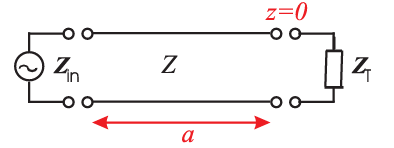
\includegraphics[width=0.5\linewidth]{input impedance.png}
            \item $V_i=V_1e^{-i(kz-\omega t)}$, $V_r=rV_1e^{-i(-kz-\omega t)}$, $\frac{V_i}{I_i}=Z$, $\frac{V_r}{I_r}=-Z$
            \item $Z_{\text{in}}=\eval{\frac{V_i+V_r}{I_i+I_r}}_{r=a}=\frac{e^{ika}+re^{-ika}}{e^{ika}-re^{-ika}}Z$, $\frac{Z_{\text{in}}}{Z}=\frac{Z_t\cos(ka)+iZ\sin(ka)}{Z\cos(ka)+iZ_t\sin(ka)}$
            \item Short-circuit, $Z_t = 0$, $\frac{Z_{\text{in}}}{Z}=i\tan(ka)$
            \item Open-circuit, $Z_t\rightarrow\infty$, $\frac{Z_{\text{in}}}{Z}=-i\cot(ka)$
            \item Quater-wavelength, $a=\lambda/4, ka=\pi/2$, $\frac{Z_{\text{in}}}{Z}=\frac{Z}{Z_t}$
        \end{itemize}
    \item (Non-TEM) Parallel plate waveguide \begin{itemize}
            \item \includegraphics*[width=0.5\linewidth]{waveguide.png}
            \item $k^2=k_x^2+k_z^2$, $k_z=k_g$, $k_x=\frac{m\pi}{a}$ (standing wave)
        \end{itemize}
    \item Rectangular waveguide\begin{itemize}
            \item General $TE_{mn}$, transverse electric, $n$ and $m$ in x,y direction
            \item $(k_x,k_y,k_z)=\left(\frac{m\pi}{a},\frac{n\pi}{b},k_g\right)$
            \item \begin{align*}
                    E_x &= A_0k_y\cos(k_x x)\sin(k_y y)\cos(k_z z-\omega t)\\
                    E_x &= -A_0k_y\sin(k_x x)\cos(k_y y)\cos(k_z z-\omega t)\\
                    E_z&=0
                \end{align*}
            \item $\frac{\omega^2}{c^2}=k_x^2+k_y^2+k_z^2$
            \item $k_z=k_g$, if imaginary, evanescent
            \item \includegraphics*[width=\linewidth]{rect_waveguide.png}
        \end{itemize}
\end{enumerate}

\end{document}